\documentclass[11pt]{article}
\usepackage[utf8]{inputenc}
\usepackage{mathtools}
\usepackage{empheq}
\usepackage{graphicx}
\usepackage{amssymb}

\title{Physique Oscillation Harmonique}
\author{Vanden Driessche Théo}

\date{November 2017}


\usepackage{geometry}
 \geometry{
 a4paper,
 total={170mm,257mm},
 left=20mm,
 top=20mm,
 }
\graphicspath{ {images/} }

\begin{document}

\maketitle

\newpage
\section{Phènomènes périodiques}
\subsection{Définitions}
-Un oscillateur est un objet décrivant un mouvement de va-et-vient de part et d'autre d'une position d'équilibre.\\
-L'élongation y d'un point P est la valeur algébrique de l'écart de P par rapport à la position d'équilibre O.

\subsection{Caractéristiques d'une oscillation}
\subsubsection{Période et fréquence}
\begin{align*}
        f&=\dfrac{1}{T} \Longleftrightarrow &T=\dfrac{1}{f} \\
        f& \Rightarrow Hz &T \Rightarrow s   
\end{align*}

\section{Mouvements Harmoniques}
\subsection{Définition}
Un mouvement harmonique est un mouvement d'oscillation dont la représentation graphique de l'élongation en fonction du temps est une sinusoïde.\\

\subsection{Amplitude}
-L'amplitude est l'écart maximal par rapport à la position d'équilibre c'est à dire l'élongation maximale. On la note A l'unité SI est le mètre (m).\\
L'amplitude correspond à la position maximale $ A = y_{(t)max}$\\
La période T coresspond au temps mis par oscillation.\\
La frequence f correspond au nombre d'oscillation par seconde.
\begin{center}
    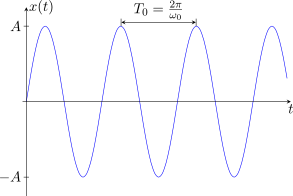
\includegraphics{oscillateur_harmonique.png}
\end{center}

\newpage
\subsection{Étude mathématique}
Supposons d'abord que la position $M_{0}$ du point M à l'instant t=0 se situe sur CX, à droite de C. L'angle $\alpha$ formé par CX et CM, qui vaut 0 à l'instant t = 0, augmente régulièrement puisque M tourne à vitesse constante.\\
La vitesse angulaire est l'angle balayé par CM par unité de temps. La notation est $\omega$. L'unité SI est le radian/seconde (rad/s).\\
$$\omega = \dfrac{\alpha}{t} \text{ ou } \alpha=\omega \cdot t$$
Projetons le mouvement de M sur un axe vertical OY. La projection P de M décrit un mouvement d'oscillation de part et d'autre de C. La valeur algébrique de CP est l'élongation. On voit que $-A \leqslant y \leqslant A $\\
La période T de P est la durée d'une oscillation complète, ce qui correspond à un tour complet. Par consequent, $\alpha _{(T)}=2\pi$.\\
Or $\alpha=\omega \cdot t$ donc $\alpha _{(T)}=\omega \cdot T = 2\pi$\\
$y_{(t)} = CP = QM = CM \cdot sin(\alpha) = A \cdot sin(\omega t)$
%\begin{gather}
 %   y_{(t)} =A\cdot sin(\alpha _{(t)}) = A\cdot sin(\omega t)    \\
  %  \omega = 2\pi f = \dfrac{2\pi}{T}
%\end{gather}
\begin{center}
    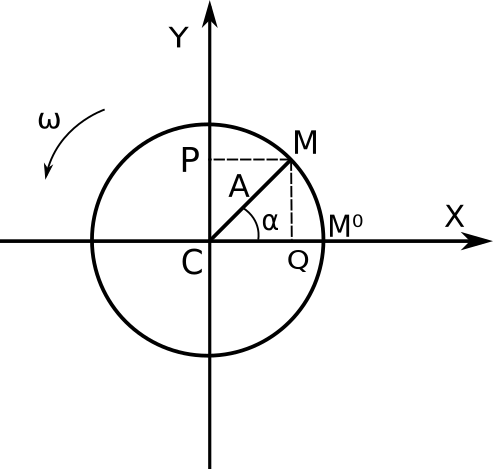
\includegraphics[scale=0.5]{Fig1_8.png}
\end{center}
\section{Dynamique}
\subsection{}

\begin{empheq}[left=\empheqlbrace]{align}
\sum F & =ma \\
 a & = -\omega ^2 y 
\end{empheq}
\begin{align*}
\Rightarrow \sum F & = -m\omega ^2 y \\
\text{ Où }  -m\omega ^2 & \text{ est constant.}
\end{align*}

\subsection{Rappel: Loi d'Hooke}
\begin{align}
    F = -kx
\end{align}
Toute force de ce type provoque un mouvement d'oscillation harmonique
par consequent:
la période peut être déduite de la relation
$$\omega = \sqrt{\dfrac{k}{m}} $$
$$T = 2 \pi \sqrt{\dfrac{m}{k}}$$
\subsection{Le pendule simple}


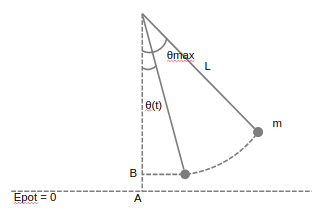
\includegraphics{testSimplePendulum.png}

Que peut faire varier la période d'un pendule simple? \\
-Son Energie de départ (E) \\
-La longeur de la corde (L) \\
-la pesanteur (g) \\

\subsubsection{Epot}
\begin{equation}
\begin{split}
    E_{tot} & = E_{pot} + E_{cin} \\
    & = mg|AB| \\
    & = mg(L-Lcos(\theta_{(t)})) \\
    & = mgL(1-cos(\theta_{(t)}))
\end{split}
\end{equation}

\subsubsection{Ecin}
\begin{align*}
E_{cin} & = \dfrac{mv^2}{2}  & v = v_{ang}L \\
&     & = \theta ' _{(t)}L & \text{ la dérivée de l'angle décrit} \\
& = \dfrac{m(\theta ' _{(t)} L)^2}{2}\\
\end{align*}

\subsubsection{Etot}
Energie totale est constante (Frottements négligeables). \\
Donc la variation d'Etot = 0. Par conséquent, sa dérivée vaux zéro.\\
$$(E_{tot})'=0$$ \\
Nous pouvons donc dire:
\begin{equation}
\begin{split}
    (E_{pot})'  & = (E_{cin} + E_{pot})' \\
    0 & = \Bigg( \dfrac{m(\theta_{(t)}' L)^2}{2} + mgL\Big(1-cos(\theta_{(t)})\Big)\Bigg)' \\
    & = \Bigg( \dfrac{m(\theta_{(t)})'^2 L^2}{2} + mgL\Big(1-cos(\theta_{(t)})\Big)\Bigg)' \\
    & = \dfrac{2}{2}mL^2 \theta_{(t)} ' \theta_{(t)}'' + mgLsin(\theta_{(t)})\theta_{(t)}' \\
    & = L \theta_{(t)}'' + y\cdot sin(\theta_{(t)}) \\
    \theta_{(t)}'' & =\dfrac{ -y\cdot sin(\theta_{(t)})}{L}
\end{split}
\end{equation}

\newpage

\begin{equation}
\begin{split}
\text{Si, } \theta < \dfrac{\pi}{6} \text{ ,on a } & sin(\theta) \cong \theta \text{ alors,}\\
\end{split}
\end{equation}
$$\theta_{(t)}'' + \dfrac{g}{L} \theta_{(t)} = 0$$ \\
Une solution de cette équation différentielle, où l'on suppose que $\omega^2 = \dfrac{g}{L}$,  est: \\
$$\theta_{(t)} = \theta_{max} sin(\omega t + \phi)$$\\
\begin{align*}
    \omega^2 & = \dfrac{g}{L} 
    & \omega = \sqrt{\dfrac{g}{L}}&
    &\dfrac{2\pi}{T}  = \sqrt{\dfrac{g}{L}}\\
    T & = \dfrac{2\pi \sqrt{\dfrac{g}{L}}L}{2}
    & T = 2\pi \sqrt{\dfrac{L}{g}} &
\end{align*}

\subsection{Energie}
\subsubsection{Énergie cinétique}
\begin{equation}
\begin{split}
    E_{cin}  = \dfrac{mv^2}{2} & = \dfrac{m\Big(\omega A \cdot cos(\omega t+ \phi)\Big)^2}{2} \\
    & =\dfrac{ m\omega^2 A^2 cos^2(\omega t+ \phi)}{2} \text{ Par l'égalité fondamentale: } \\
    & = \dfrac{ m\omega^2 A^2 \Big(1-sin^2(\omega t+ \phi)\Big)}{2} \\
    & =\dfrac{m\omega^2\Big(A^2-A^2sin^2(\omega t+ \phi)\Big)}{2} \\
    & =\dfrac{m\omega^2(A^2-y_{(t)}^2)}{2} \\
    & = \dfrac{k(A^2-y_{(t)}^2)}{2}
\end{split}
\end{equation}
\subsubsection{Énergie totale}
 L'énergie totale est égale à l'énergie cinetique lorsque $y_{(t)}=0$ \\
 \begin{equation}
     \begin{split}
         E_{tot} & = E_{cinMax}\\
        & = \frac{kA^2}{2}
     \end{split}
 \end{equation}
\subsubsection{Énergie potentielle élastique}
Par définition, $E_{pot} = E_{tot}-E_{cin}$ \\
\begin{equation}
    \begin{split}
        E_{pot} & = E_{tot}-E_{cin} \\
        & = \frac{kA^2}{2} - \dfrac{k(A^2-y_{(t)}^2)}{2} \\
        & = \frac{k(A^2-A^2+y_{(t)}^2)}{2} \\
        & = \frac{ky_{(t)}^2}{2}
    \end{split}
\end{equation}

\end{document}
